\chapter{Initital Stages of Heat Generation: Electron-phonon Thermalization in Nanoscale Systems}	% Chapter 2.

Work presented in this chapter is adapted from the following paper:

\begin{itemize}
\item Hannah, D. C.; Brown, K. E.; Young, R. M.; Wasielewski, M. R.; Schatz, G. C.; Co, D. T.; Schaller, R. D. \emph{Phys. Rev. Lett.} \textbf{2013}, 111, 107401
\end{itemize}

Theoretical work in this chapter is adapted, in part, from the following paper:

\begin{itemize}
\item Aruda, K. O.; Tagliazucchi, M.; Sweeney, C. M.; Hannah, D. C.; Schatz, G. C.; Weiss, E. A. \emph{Proceedings of the National Academy of Sciences} \textbf{2013}, 110, 4212–4217.
\end{itemize}

\section{Overview}

Subsequent to the excitation of charge carriers, often by an applied electromagnetic field, excited electrons and holes dissipate energy by thermalizing with vibrational degrees of freedom in the host lattice as well as the surrounding environment (such as ligand and solvent/matrix vibrations). Such thermalization processes are a key energy loss mechanism in semiconductor materials and a contributor to heat generation, so controlling these processes is of technological interest. While carrier thermalization has been studied extensively in bulk materials and for over a decade in nanomaterials, several open questions remain. As discussed in Chapter 1, the absence of a theoretically predicted phonon bottleneck in strongly-confined semiconductor NCs has stimulated a body of work attempting to resolve the true nature of carrier energy loss mechanisms in these materials. The prevailing interpretation of carrier thermalization invokes Auger-like energy transfer between the electron and hole (as discussed in Chapter 1). However, Auger-like energy transfer remains unproven, and several recent experimental results call this explanation into question. For example, removal of the hole (which nominally receives energy from the electron, facilitating electron cooling) does not significantly slow electron cooling rates \cite{PhysRevB.60.R2181, klimov2000mechanisms}. Furthermore, materials exhibiting similar carrier effective masses, such as PbSe, also exhibit subpicosecond carrier cooling despite the expectation that Auger-like energy transfer should not productively yield carrier cooling in such materials \cite{wehrenberg2002interband, harbold2005time}. These results would seem to suggest that multi-phonon transitions somehow become significantly more efficient or that higher-energy ligand vibrations are able to participate in the carrier thermalization process. \par

Direct examinations of phonon generation during NC carrier cooling remain missing from the literature, despite the evident importance of this process to understanding carrier energy loss in NCs. In this Chapter, we first detail the experimental setups and methods used to characterize ultrafast processes in NCs throughout this thesis. \par

Next, we report femtosecond stimulated Raman spectroscpoy measurements of lattice dynamics in semiconductor nanocrystals and characterize longitudinal optical (LO) phonon production during confinement-enhanced, ultrafast intraband relaxation. Stimulated Raman signals from unexcited CdSe nanocrystals produce a spectral shape similar to spontaneous Raman signals. Upon photoexcitation, stimulated Raman amplitude decreases owing to experimentally resolved ultrafast phonon generation rates within the latice. We find a $\sim$600 fs, particle-size-independent depletion time attributed to hole cooling, evidence of LO-to-acoustic down-conversion, and LO phonon mode softening. \par

Finally we briefly consider the role played by surface ligands in mediating analogous processes (hot electron cooling) in similarly-sized metallic nanoparticles. Specifically, we report density functional theory (DFT)-derived electronic structure calculations on thiol- and amine-passivated gold slabs. We find that thiol-functionalization greatly increases the density of electronic states near the gold Fermi level as compared to the aminated case, resulting in elevated electronic heat capacity. This elevated electronic heat capacity manifests as a longer hot electron lifetime, which is observed using transient absorption spectroscopy.

\section{Experimental Characterization of Carrier Cooling in Semiconductor Nanocrystals}

As discussed in the introductory Chapter of this thesis, intraband relaxation in NCs generally proceeds on a sub-picosecond timescale. Therefore characterization of the carrier cooling process is typically accomplished using time-resolved optical spectroscopy, which is capable of providing the extremely high time-resolution required. The work presented in this Chapter makes use of two spectroscopic pump-probe techniques sensitive to dynamics on these timescales: Transient absorption spectroscopy (TA) and femtosecond stimulated Raman spectroscopy (FSRS). We briefly review each technique and the experimental setups we utilized here.

\subsection{Transient Absorption Spectroscopy}
\subsubsection{Overview}
In transient absorption spectroscopy, two ultrashort pulses ($< 50$ fs) are used to study the dynamic evolution of a sample absorption spectrum. The first pulse, termed the pump pulse, initiates a time-dependent process in the sample. A mechanically delayed second pulse, termed the probe pulse, interrogates the sample absorption spectrum at various times subsequent to photoexcitation. The nature of these pulses can vary according to experimental needs; we will review our setup in the next section. The transient absorption spectrum is calculated according to Equation \ref{eq:ta1}:
\begin{equation}\label{eq:ta1}
\Delta OD(\lambda, t) = OD(\lambda, t)_{ON} - OD(\lambda, t)_{OFF} = \log{\frac{I(\lambda, t)_{OFF}}{I(\lambda,t)_{ON}}}
\end{equation}
"ON" and "OFF" refer to probe spectra collected with and without the pump pulse.  These spectra are generally obtained by mechanically chopping the pump pulse.
\subsubsection{Experimental TA apparatus}

\begin{figure}
\begin{center}
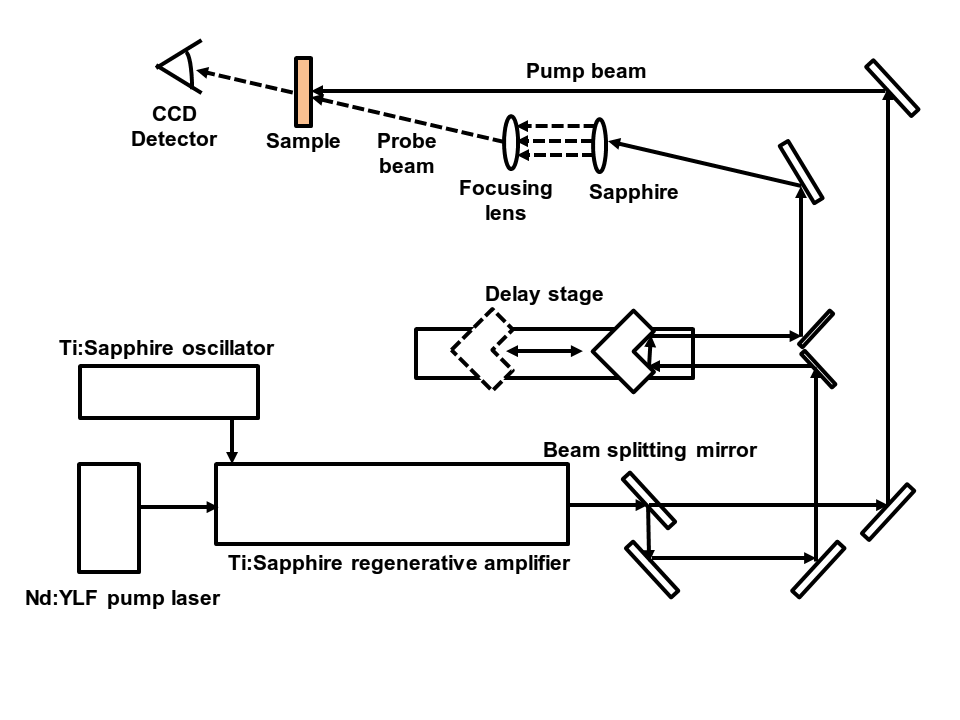
\includegraphics[width=\textwidth]{./Chapter2/ta_setup.png}
\caption[Block diagram of transient absorption apparatus.]{Block diagram of the experimental appartus used to collect the transient absorption and time-resolved PL data presented in this work.}
\label{f:tasetup}
\end{center}
\end{figure}

Unless otherwise noted, the transient absorption measurements described in this work were carried using the apparatus depicted in Figure \ref{f:tasetup}. A regeneratively amplified Ti:Sapphire laser operating at a 2-kHz repitition rate was used to generate 35 fs pulses with a wavelength of 800 nm. A portion (5\%) of the amplifier output was time-delayed and focused onto a sapphire plate to produce a white-light probe pulse. The remaining output was either frequency-doubled to 400 nm or used to feed an optical parametric amplifier (OPA) for spectrally tunable pump pulses. Pump and probe pulses were overlapped on the sample, and pump pulses were mechanically chopped at a frequency of 1 kHz.

\subsubsection{Special Considerations for Nanocrystals}
One of the most important features of the transient absorption spectrum of CdSe nanocrystals is the $1S_{3/2}-1S_e$ bleach, corresponding to the band-edge exciton. In nanocrystals, state filling leads to bleaching of the interband transitions between populated quantized states \cite{doi:10.1021/jp9944132}. \par

The valence band in CdSe nanocrystals is 3-fold degenerate. Additionally, the hole in this material exhibits a much larger effective mass than the electron such that $m_h/m_e \approx 6$. Because of this, the thermal occupation probabilities of electron states are far greater than those of the coupled hole states. Put simply, the thermal distribution of hole populations is spread over many levels. A consequence of this asymmetry between electron and hole populations is that the $1S_{3/2}-1S_e$ bleach feature in TA spectra is sensitive primarily to electron populations \cite{doi:10.1021/jp9944132}. 

\subsection{Femtosecond Stimulated Raman Spectroscopy}
\subsubsection{Overview}
Similar to transient absorption spectroscopy, the femtosecond stimulated Raman spectroscopy (FSRS) process begins with an ultrashort laser pulse, termed here the actinic pulse, which initiates a time-dependent process in the sample of interest. The evolution of the structure and vibrational populations of the system are interrogated after a time delay by a pair of pulses which drive stimulated Raman transitions in the sample: a narrow bandwidth, temporally broad Raman pulse and short broadband probe pulse. When these two pulses are simultaneously incident on the sample, Raman transitions having a frequency of $\omega_v = \omega_{Probe} - \omega_{Raman}$ cause a net attenuation of the pump beam and net gain in the probe beam. The final Raman scattering spectrum is obtained by dividing out a probe spectrum without a co-incident Raman pump pulse, similar to the pump-off/pump-on motif shown in Eq. \ref{eq:ta1}, but with the Raman pulse being mechanically chopped \cite{doi:10.1146/annurev.physchem.58.032806.104456}. \par

The time resolution of FSRS is determined only by the duration of the actinic and Raman pump pulses. The detection of FSRS is not time-resolved, and so the frequency resolution of FSRS is independent of the time-energy Fourier limitations of the femtosecond pulses. Thus, FSRS is one of the only techniques capable of probing the dynamics of low-frequency vibrations on sub-picosecond timescales. This makes it ideally suited to the examination of the role played by (low-frequency) phonons in NC intraband carrier cooling.

\subsubsection{Experimental FSRS Apparatus}

\begin{figure}
\begin{center}
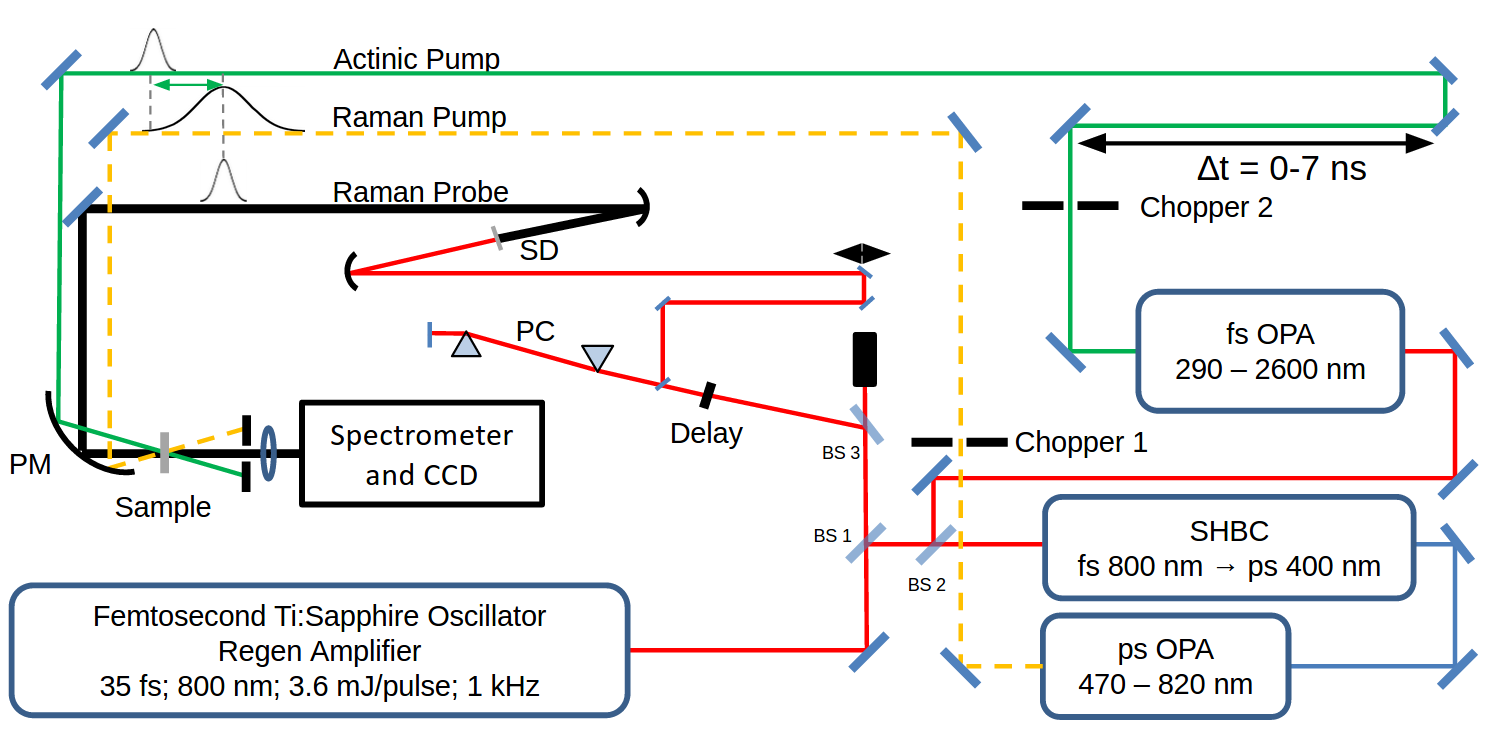
\includegraphics[width=\textwidth]{./Chapter2/fsrs_setup.png}
\caption[Block diagram of femtosecond stimulated Raman spectroscopy apparatus.]{Block diagram of the experimental apparatus \cite{doi:10.1021/jz301107c} used to collect the femtosecond stimulated Raman spectroscopy data presented in this Chapter.  Reproduced from Ref. 15.}
\label{f:fsrssetup}
\end{center}
\end{figure}

Figure \ref{f:fsrssetup} displays the experimental setup utilized here for the acquisition of FSRS data. The 800 nm, 35-fs pulse output of regeneratively amplified Ti:Sapphire laser operating at 1 kHz is split first using a 80\% reflective beamsplitter (BS1 in Fig. \ref{f:fsrssetup}). The transmitted portion is is directed to a second beamsplitter (BS3), which transmits 10\% of the remaining output to a sapphire disk in order to produce the white light probe pulse. The reflected portion of the initial amplifier output is sent through a 50\% beam splitter (BS2). The transmitted portion is frequency doubled with a second harmonic bandwidth compressor (SHBC) to give a 400-nm pulse. This pulse is used to seed a narrow bandwidth ps-OPA, which provides a spectrally tunable Raman pulse. The reflected portion is directed to a second, femtosecond OPA to produce short, spectrally tunable actinic pump pulses. Time delay between the actinic pump and Raman/probe pulse pair is controlled \emph{via} a motorized delay stage in the actinic pump beam path. The Raman pulse is chopped at a frequency of 125 kHz to obtain pump on and pump off spectra. The full details of this setup are reported in work by Brown \emph{et al.} \cite{doi:10.1021/jz301107c}

\section{Basic Characterization of CdSe Nanocrystals}
The CdSe nanocrystals utilized in the experiments reported in this Chapter (as well as Chapter 3) were examined by absorption spectroscopy as well as transmission electron microscopy in order to characterize particle size and shape. Figure \ref{f:basic1} displays the static UV-visible absorption spectrum of various CdSe NC sizes suspended in hexane. The spectra exhibit (expected) features characteristic of quantum confinement, including a sharp excitonic peak and size-dependent absorption onsets. 

\begin{figure}
\begin{center}
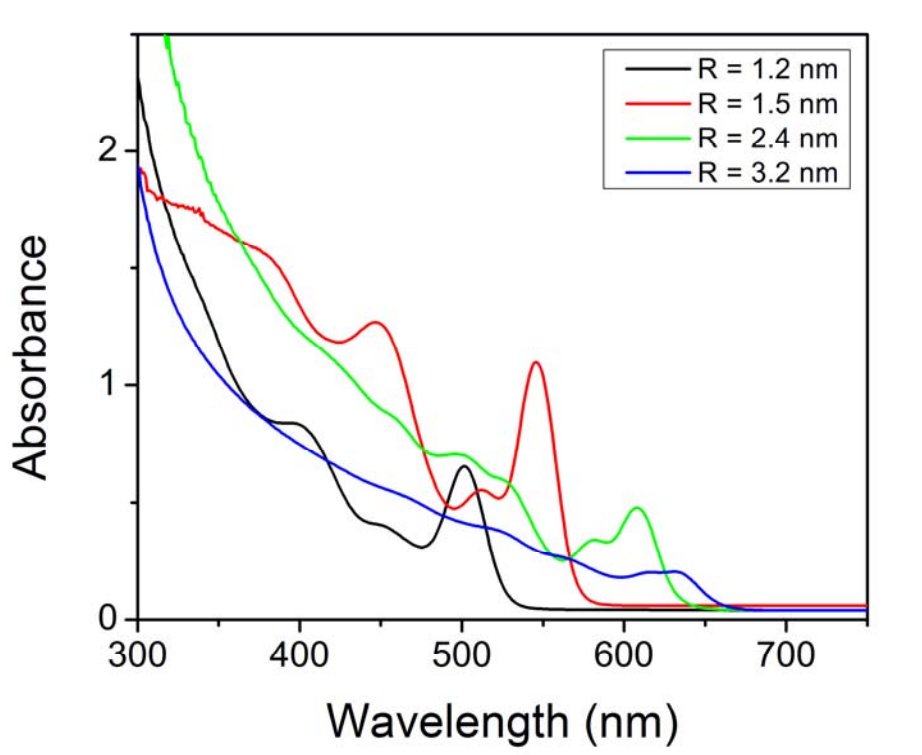
\includegraphics[width=0.75\textwidth]{./Chapter2/basic1.png}
\caption[Absorption spectra of CdSe NC samples examined in this work.]{UV-visible absorption spectra of four sizes of CdSe NC suspended in hexane.  Average particle radii are indicated in the figure legend.}
\label{f:basic1}
\end{center}
\end{figure}

Figure \ref{f:basic2} shows a transmission electron micrograph of CdSe collected on an amorphous carbon substrate. These particles are spherical in shape an exhibit the wurtzite crystal structure.

\begin{figure}
\begin{center}
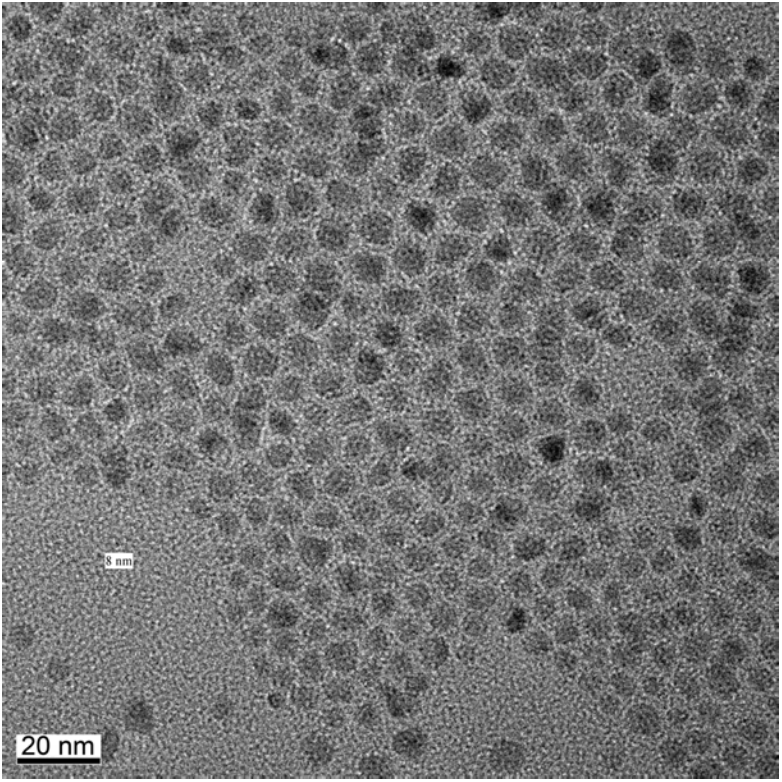
\includegraphics[width=0.75\textwidth]{./Chapter2/basic2.png}
\caption[Transmission electron micrograph of CdSe NCs.]{Transmission electron micrograph of CdSe nanocrystals.}
\label{f:basic2}
\end{center}
\end{figure}


\section{Direct Characterization of Lattice dynamics in Semiconductor Nanocrystals Using FSRS}

As noted above, confinement-enhanced electron-to-hole Auger energy transfer has been suggested as the primary means of hot exciton cooling in CdSe NCs where electron excess energy is transferred to holes that then rapidly cool via phonon emission \cite{Efros1995281}.  Experimentally, transient absorption (TA) measurements show faster intraband exciton cooling in smaller particles with larger bandgaps \cite{PhysRevB.60.13740, PhysRevB.60.R2181, PhysRevLett.80.4028}, consistent with the proposed mechanism. Since bleach signals in CdSe NCs predominantly arise from excited electrons, these measurements specifically convey NC size-dependent electron cooling rates \cite{Wang23032001, doi:10.1021/ja070099a, doi:10.1021/jp9944132}.  Recently, Xu \emph{et al.} observed rapid hole cooling times via comparison of TA and femtosecond up-conversion measurements \cite{PhysRevB.65.045319}.  Similarly, Hendry et al. measured the non-resonant transient conductivity of photo-excited NCs using terahertz time-domain spectroscopy and reported a $\sim$1 ps electron-hole coupling time \cite{PhysRevLett.96.057408}.  Missing from the literature are direct examinations of lattice dynamics during this process. Such measurements present inherent challenges as the typical sub-picosecond carrier relaxation lifetimes and small phonon energies obviate the utility of transient spontaneous Raman spectroscopy \cite{PhysRevB.80.121403}.  \par

We utilized FSRS, notable for the high temporal ($\sim$100 fs) and energy ($\sim$10 cm$^{-1}$) resolution described above \cite{doi:10.1146/annurev.physchem.58.032806.104456}, to investigate phonon dynamics in photoexcited NCs for the first time.  For CdSe NCs, we observe sub-picosecond phonon dynamics along with mode softening, and note a lack of size dependence for the initial change in signal levels despite size-dependent electronic intraband relaxation \cite{Wang23032001, doi:10.1021/ja070099a, doi:10.1021/jp9944132}.  We attribute the initial FSRS depletion time constant to size-independent hot-hole-to-phonon coupling. We also observe a rapid ($\tau$ = $\sim$2 ps) recovery of the stimulated Raman signal that is consistent with relaxation of LO phonon populations into other vibrational modes.  This rapid phonon downconversion is followed by a slower recovery of gain amplitude with a timescale and size-dependence consistent with phonon outflow from the NC into the surrounding matrix. Diminished gain amplitude at even longer times ($\sim$1 ns) is suggestive of persistent LO-phonon generating processes or altered phonon coupling in NCs containing a band-edge exciton, for which the radiative lifetime is on the order of nanoseconds. \par

We examine hexane suspensions of octadecylamine-capped CdSe NCs with spherical particle shapes, and optical properties as noted in Qu \emph{et al.} \cite{doi:10.1021/ja017002j}.  Figure \ref{f:fsrs1} shows a schematic depicting the FSRS experiment in the context of NC dynamics.  The details of the experimental setup are reported above and elsewhere \cite{doi:10.1021/jz301107c}.  Here, we adjust the actinic and Raman pump fluences such that the average number of electron-hole pairs generated per NC is less than 0.2 \cite{doi:10.1021/jp9944132}.  This assures that dynamics related to single excitons are observed. Optical Kerr-effect (OKE) cross-correlation of the actinic pump and probe pulses in hexane indicates a time resolution of $\sim$170 fs. \par

\begin{figure}
\begin{center}
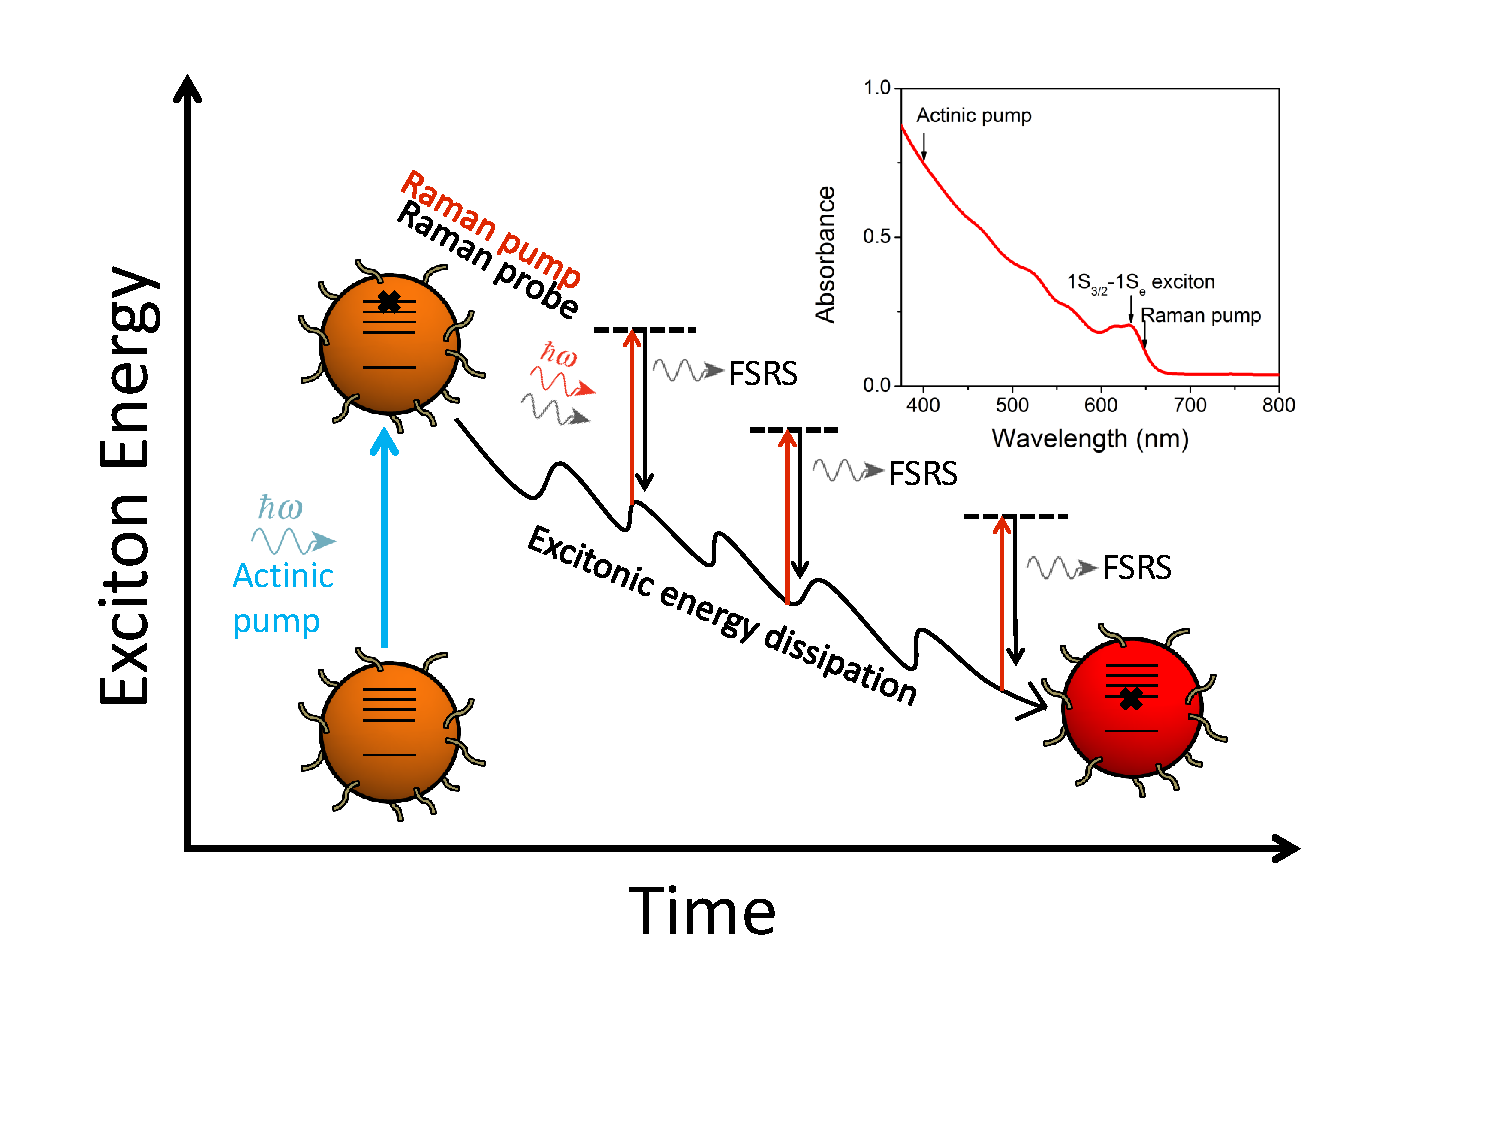
\includegraphics[width=\textwidth]{./Chapter2/fsrs1.pdf}
\caption[Diagram demonstrating the application of FSRS to exciton cooling in NCs.]{An actinic pump photon, having energy greater than the NC energy gap, excites a hot electron-hole pair, denoted by ‘X’.  The ladder levels represent exciton (\emph{i.e.} electron + hole) states.  As the system evolves in time, hot carriers cool via various pathways including phonon emission and Auger-like electron-to-hole energy transfer.  The Raman pump, which is resonant with electronic transitions in the NC, and probe pulses stimulate Raman transitions at various time delays, generating FSRS signal. Inset: Absorption spectrum of 3.1-nm radius CdSe nanocrystals capped with octadecylamine and suspended in hexane.  The actinic pump and Raman pump wavelengths are indicated relative to the 1S$_{3/2}$-1S$_e$ exciton transition.}
\label{f:fsrs1}
\end{center}
\end{figure}

Figure \ref{f:fsrs2}(a) displays raw FSRS spectra of colloidal CdSe NCs with a 1.5 nm radius. The features observed are consistent with previous static measurements of resonant Raman scattering in this material \cite{aliviresodepolar}.  The peak at $\pm$210 cm$^{-1}$ corresponds to the longitudinal optical (LO) phonon mode of the CdSe lattice and a 2LO phonon Raman peak also appears at $\pm$410 cm$^{-1}$.  Atypically, the CdSe phonon features exhibit gain at both Stokes and anti-Stokes frequencies.  A low-frequency shoulder on the LO phonon feature, commonly observed in spontaneous Raman and attributed to the surface optical (SO) phonon mode \cite{aliviresodepolar, DzhaganPhonon} is reproducibly observed both here (Fig. \ref{f:fsrs2}(a), inset) as well as in static Raman spectra.  To analyze each mode, we fit the LO phonon feature using the sum of two Gaussians as illustrated in the inset of Fig. 2(a). In the dynamics experiments discussed later in this report, we note that the LO and SO phonon modes exhibit indistinguishable dynamics, suggestive of a single population exhibiting both phonon features. \par

\begin{figure}
\begin{center}
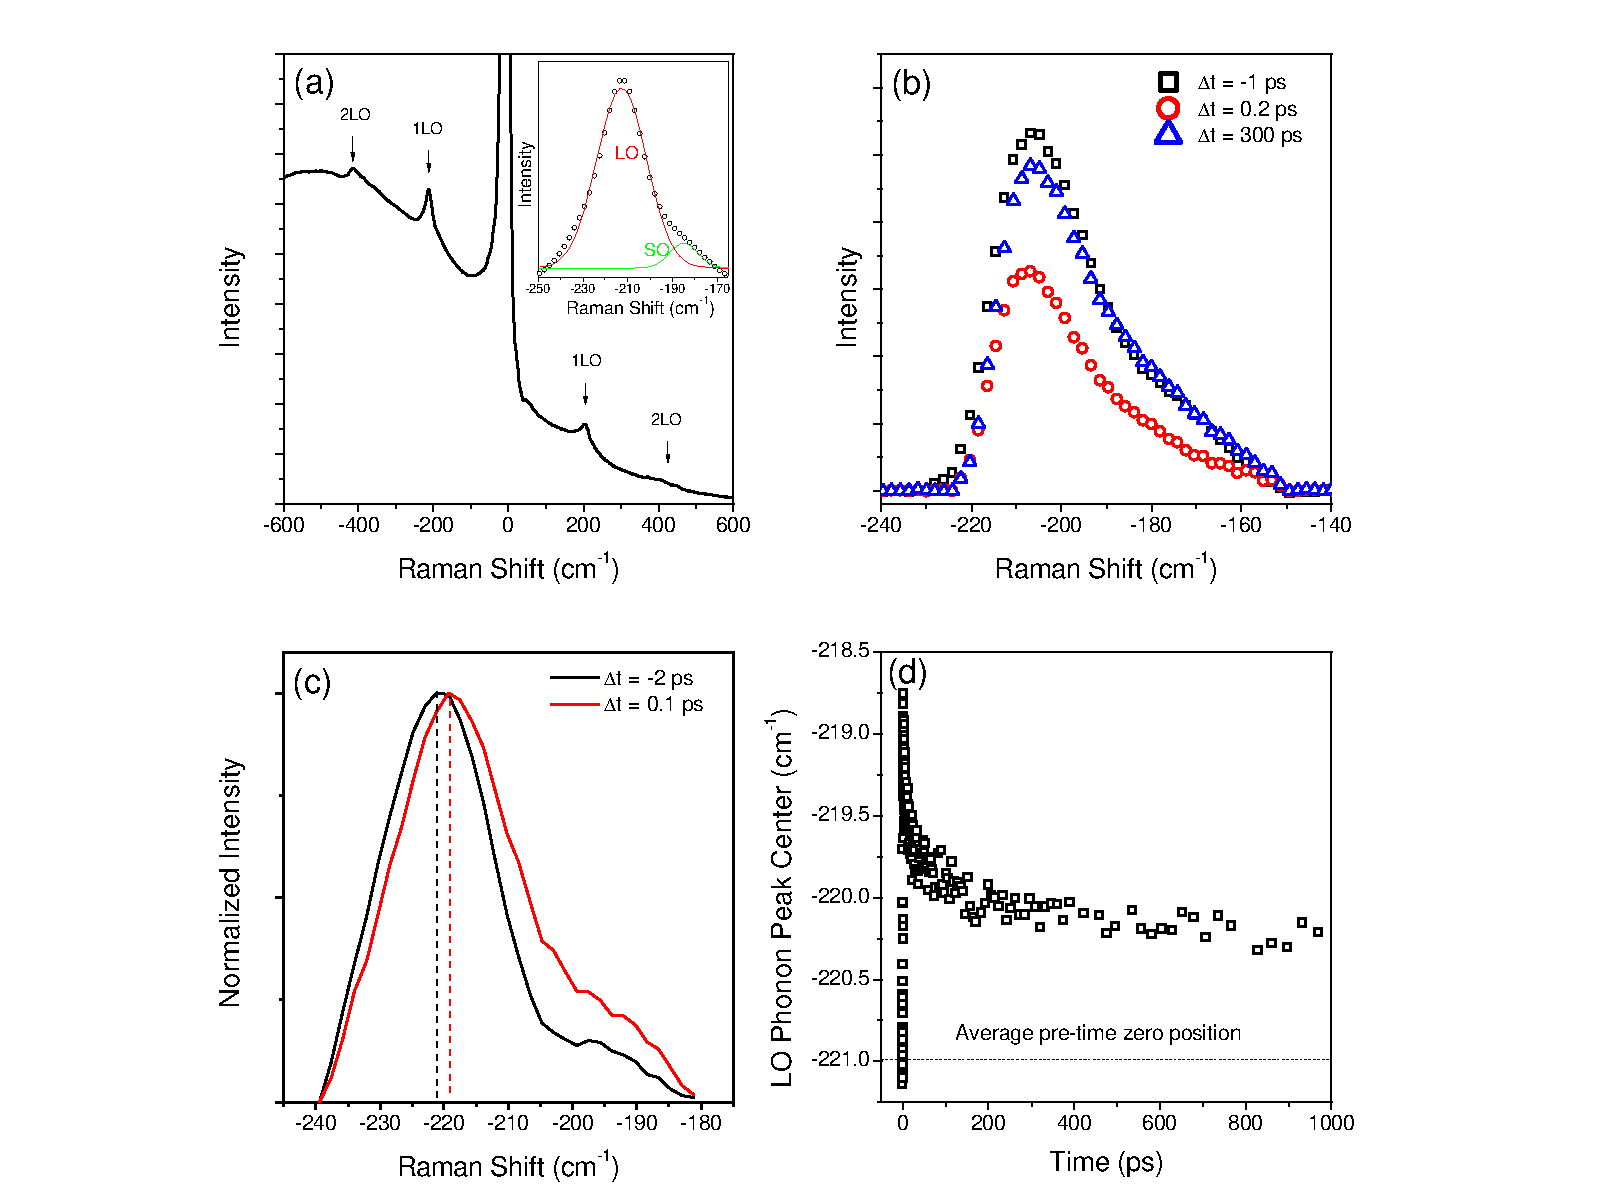
\includegraphics[width=\textwidth]{./Chapter2/fsrs2.pdf}
\caption[Features of FSRS spectra of CdSe NCs.]{(a) Raw ground-state FSRS spectrum for 3.1 nm radius CdSe NCs suspended in hexanes at negative time delay (prior to photoexcitation by the actinic pump). 1LO and 2LO phonon features are indicated. The inset displays a fit of the background-subtracted anti-Stokes peak to the sum of two Gaussian functions. The blue line indicates the overall fit. In accordance with previous reports, the Gaussian function given in red is assigned to the LO phonon mode, while the blue Gaussian function is assigned to the SO phonon mode. (b) Background-subtracted anti-Stokes phonon peak for 3.1-nm radius CdSe NCs at indicated pump probe time-delays. (c) Normalized anti-Stokes phonon band for a 2.4-nm radius CdSe NC at the indicated time delays. The color-coded dotted line serves as a guide to the eye and represents the location of the LO phonon peak center as determined by fits of the phonon band to two Gaussian functions. (d) Dynamics of the LO phonon peak center for a 2.4-nm radius CdSe NC derived from the two-Gaussian fit. The location of the phonon peak center prior to photoexcitation is indicated by the dotted black line.}
\label{f:fsrs2}
\end{center}
\end{figure}

Figure \ref{f:fsrs2}(b) shows background-subtracted time-resolved spectra for the anti-Stokes 1LO phonon feature at three time delays relative to the 0.5 nJ/cm$^2$ actinic pump: Both the Stokes (not shown) and anti-Stokes gain amplitudes are depleted by photoexcitation, with partial recovery of the gain signal at longer times. Normalized, background-subtracted 1LO phonon FSRS spectra, presented in Fig. \ref{f:fsrs2}(c) for a 2.4 nm radius CdSe NC, prior to (-2 ps) and shortly after (0.1 ps) photoexcitation reveal that the 1LO phonon feature is red-shifted by approximately 2 cm$^{-1}$ for both the Stokes and anti-Stokes features. This redshift occurs upon generation of LO phonons by photoexcited NCs. The presence of excitons in NCs leads to a transient renormalization (softening) of the LO phonon frequency. To explain this, we consider the exciton-phonon interaction due to Frolich coupling. The general form of this interaction is shown in Equation \ref{eq:fsrs_eq1} \cite{PhysRevLett.80.3105}:
\begin{equation} \label{eq:fsrs_eq1}
H_{ex-LO} = \sum_{ij}\sum_{nlm}\gamma_{nlm}^{ij}c_i^{\dagger}c_j\left(a_{nlm}^{\dagger}+a_{nlm}\right)
\end{equation}
where $c_i$ denotes the annihilation operator for the $i$th exciton state $a_{nlm}$ is the phonon annihilation operator for the $n$th phonon having angular momentum $l$.  $\gamma_{nlm}^{ij}$ are the exciton-phonon coupling matrix elements.  In the case of strongly confined NCs (including CdSe), excitons couple strongly to LO phonons having $l = 0$ and their coupling can be expressed in terms of sine integrals \cite{1996JETP...83..610F}.  The form of the exciton-phonon matrix elements is given by Equation \ref{eq:fsrs_eq2}:
\begin{equation} \label{eq:fsrs_eq2}
\begin{split}
\gamma_{nlm}^{ij} =& -e\sqrt{\frac{\Omega}{\kappa R}}\left[\mathrm{Si}\left(\left(n+i-1\right)\pi\right) - \mathrm{Si}\left(\left(n+i+1\right)\pi\right)\right. \\
&+ \left.\mathrm{Si}\left(\left(n-i+1\right)\pi\right) - \mathrm{Si}\left(\left(n-i-1\right)\pi\right) \right]
\end{split}
\end{equation}
where, in this equation only, "Si" (not to be confused with silicon) denotes the sine integral, $\Omega$ is the Lo phonon frequency, and $\kappa = \frac{\epsilon_0\epsilon_\infty}{\epsilon_0 - \epsilon_\infty}$.  Once the coupling constants are obtained, the change in the phonon frequency for an excited NC may be calculated using second-order perturbation theory following the procedure described by Zimin \emph{et al.} \cite{PhysRevLett.80.3105}:
\begin{equation} \label{eq:fsrs_eq3}
\mathrm{d}\Omega = -\sum_{i \neq 0}\frac{|\gamma_n^{0i}|^2 2\left(E_i - E_0\right)}{\left(E_i - E_0\right) - \Omega^2}
\end{equation}
In Equation \ref{eq:fsrs_eq3}, $E_i$ denotes the energy of the $j$th exciton state.  Using Equations \ref{eq:fsrs_eq2} and \ref{eq:fsrs_eq3}, we carry out this analysis using CdSe material parameters.  For a 2.4-nm radius CdSe NC, we estimate a change in LO phonon frequency upon photoexcitation of -2.6 cm$^{-1}$, in good agreement with our observation.  Fig. \ref{f:fsrs2}(d) displays the dynamics of the LO phonon peak center for the same sample.  Following the initial red-shift, the 1LO phonon peak center shifts back towards its original position, but remains slightly red-shifted even at time delays of 1 ns, likely owing to a long-lived population of single excitons in photoexcited NCs. \par

\begin{figure}
\begin{center}
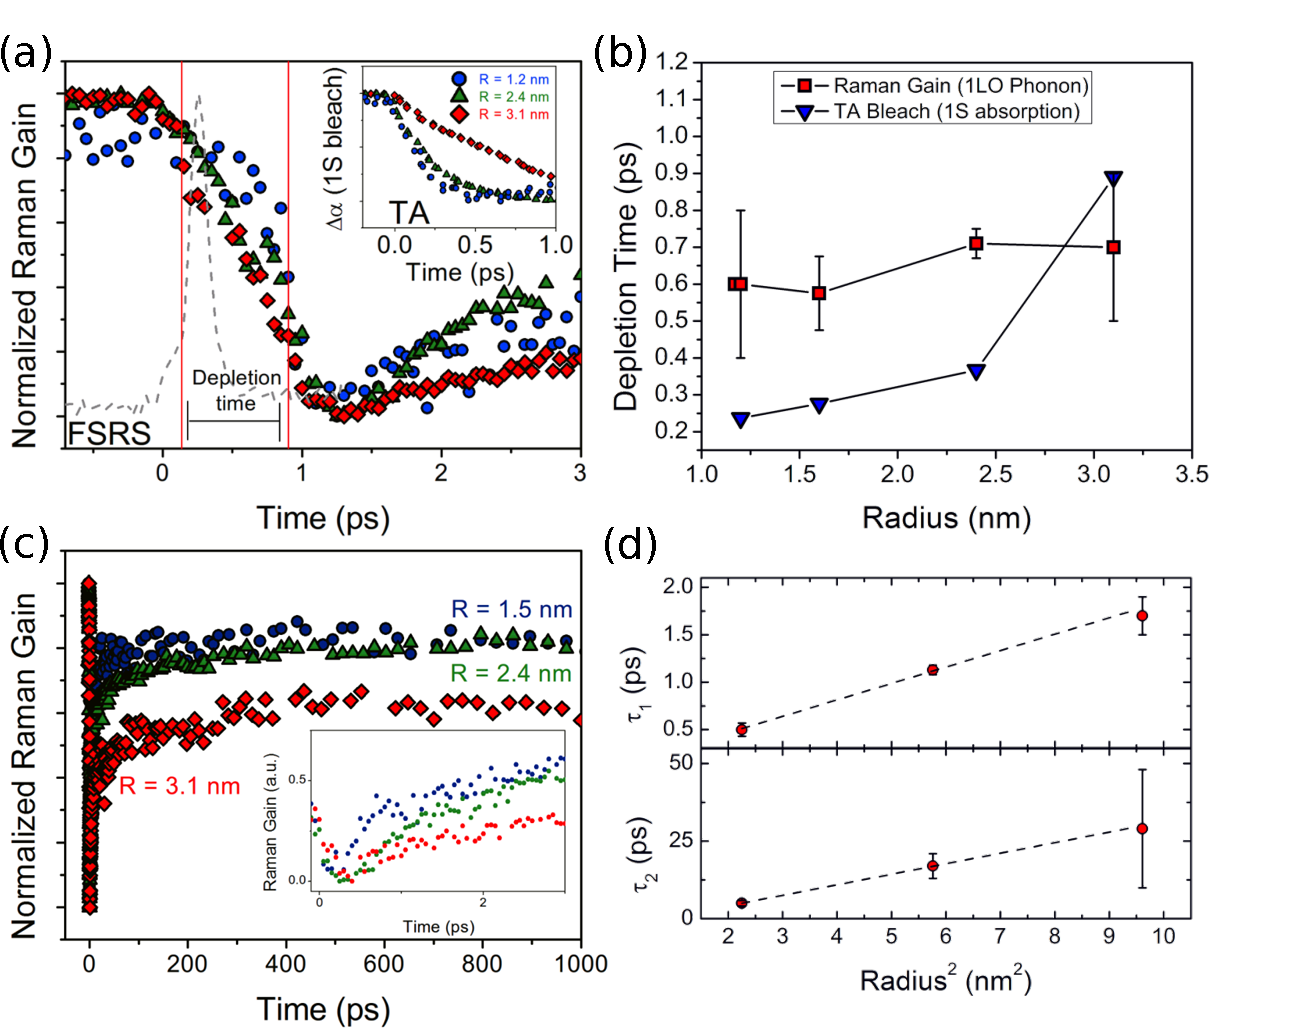
\includegraphics[width=\textwidth]{./Chapter2/fsrs3.pdf}
\caption[FSRS dynamics for a variety of CdSe NC sizes.]{(a) Anti-Stokes gain amplitude dynamics at the 1LO phonon frequency for CdSe NCs having radii of 1.2 nm (blue circles), 2.4 nm (green triangles), and 3.1 nm (red diamonds). Data are presented for time delays corresponding to the first few picoseconds
before and after the actinic pump arrival ($\Delta t = 0$).  The dotted gray line shows the IRF.  The vertical red lines indicate the signal depletion time, defined here as the time taken for the signal to drop from 80\% to 20\% of its initial ($\Delta t < 0$) intensity.  The inset displays transient absorption dynamics of the $1S_{3/2}-1S_e$ bleach feature for the same set of NCs.  (b) Anti-Stokes gain amplitude dynamics for 1.5 nm (navy circles), 2.4 nm (green triangles) and 3.1 nm (red diamonds) radius CdSe NCs at time delays up to 1 ns.  The inset shows the same dynamics for time delays from 0 to 12 ps.  (c) Comparison of measured depletion times for the FSRS 1LO phonon anti-Stokes gain feature (crosses) and the $1S_{3/2}-1S_e$ exciton bleach formation time constants (triangles) as a function of NC radius.  Error bars represent the standard deviation from multiple measurements, when available. (d) Time constants acquired from fitting the post-depletion FSRS signal to a tri-exponential recovery function. Error bars are derived from the standard deviations of repeat measurements when available.}
\label{f:fsrs3}
\end{center}
\end{figure}

In Fig. \ref{f:fsrs3} we present FSRS dynamics as a function of pump-probe delay for several NC sizes. Fig. \ref{f:fsrs3}(a) displays the temporal evolution of the 1LO phonon Stokes signal amplitude for the first few picoseconds. Comparison of the instrumental response function (IRF) to the transient phonon signal indicates that the initial dynamical changes in stimulated Raman intensity are well-resolved. The early-time FSRS data are dominated by a rapid depletion of the 1LO phonon peak amplitude followed by a slower recovery. Expressions found in the work of Eesley and later McGrane \emph{et al.} \cite{Eesley1979507, PhysRevLett.107.043001} indicate that stimulated Raman scattering intensity depends exponentially on the inverse of the LO phonon occupation number. FSRS gain intensity can be described by:
\begin{equation} \label{eq:fsrs_eq4}
I\left(\omega_{gain}, L\right) = I\left(\omega_{gain}, 0\right)e^{\frac{C_{gain}}{n + 1}}
\end{equation}
In Equation \ref{eq:fsrs_eq4}, $C_{gain}$ is a collection of terms that depend weakly on temperature; $C_{gain} = \left[I(\omega_1)\partial^2\sigma_R/\partial\omega\partial\Delta\omega\right] \times \left(\pi c^4 L \mu_0/8\hbar\omega_{gain}^3 n_1 n_{gain} \varepsilon_0\right)$.  Here, $L$ is the sample length, $\omega_1$ and $\omega_{gain}$ are the Raman pump and gain frequency, respectively, $n_1$ and $n_{gain}$ are the refractive indices of the sample at $\omega_1$ and $\omega_{gain}$, and $n$ is the Bose-Einstein phonon occupation number, given by $n = \exp\left[\left(\omega_{LO}/k_BT\right) - 1\right]^{-1}$.  Such a dependence taken together with the reduced stimulated Raman gain following excitation strongly suggests that the LO phonon population within the NCs increases following excitation.  \par

Fig. \ref{f:fsrs3}(b)  shows FSRS data for three NC sizes at probe delays up to 1 ns in the main panel, with an intermediate time scale (out to 12 ps) shown in the inset. The data in Fig. \ref{f:fsrs3}(b) show a recovery of the depleted LO phonon gain amplitude, indicative of decreased LO phonon occupation number with time. The recovery dynamics (following the Raman gain minimum) exhibit a rapid initial component followed by two slower recovery components. Time constants extracted from triexponential fitting are shown in Table \ref{table:fsrsT1} for three NC sizes [Fig. \ref{f:fsrs3}(b)]. \par

\begin{table}
\caption{Time constants for Raman gain recovery dynamics extracted from fits to a triexponential function. Errors are derived from the triexponential fits.}
\centering
\begin{tabular}{c r r r}
\hline\hline
Radius (nm) & $\tau_1$ (ps) & $\tau_2$ (ps) & $\tau_3$ (ps) \\
\hline
1.5 & 0.50 $\pm$ 0.07 & 5.0 $\pm$ 0.9 & 104 $\pm$ 34 \\
2.4 & 1.13 $\pm$ 0.05 & 17 $\pm$ 4 & 229 $\pm$ 43 \\
3.1 & 1.7 $\pm$ 0.2 & 29 $\pm$ 19 & 200 $\pm$ 82 \\
\hline
\end{tabular}
\label{table:fsrsT1}
\end{table}

Figure \ref{f:fsrs3}(d) displays recovery time constants as a function of NC size. Specifically, both $\tau_1$ and $\tau_2$ display a linear dependence on the squared NC radius. The fast Raman gain recovery component ($\tau_1$) exhibits a picosecond time constant that is consistent with the decay of LO phonons into acoustic phonon modes, based upon previous estimates that utilized resonance Raman linewidth analysis \cite{:/content/aip/journal/jcp/98/11/10.1063/1.464501} [Fig. \ref{f:fsrs3}(b), inset].  Recent theoretical studies predict similar time scales for optical phonon relaxation in other materials \cite{0295-5075-101-1-16001}.  This initial rapid recovery exhibits a dependence on NC size, with smaller NCs recovering more rapidly. Similar size dependence is observed for the intermediate component ($\tau_2$).  Along with the observed dependence on NC radius, these intermediate time constants ($\tau_2 = \sim 2 - 20$ ps) resemble previously reported time scales for the thermalization of the NC with the surrounding medium \cite{PhysRevLett.107.177403}, but as that work measures thermal transport due to \emph{acoustic} phonons, further study will be needed to definitively assign the origin of these dynamics. The slowest component of the recovery ($\tau_3$) exhibits time constants ranging from $\sim$100 - 230 ps.  The time scale of the slower recovery as well as the lack of complete recovery by 1 ns precludes intraband relaxation or biexcitonic Auger recombination, but is consistent with nanosecond time scale recombination (radiative and nonradiative) of excitons and trions \cite{:/content/aip/journal/apl/82/17/10.1063/1.1570923, doi:10.1021/nn9001177}.  The influence of carrier recombination on these processes suggests a contribution to the FSRS signal by photoexcited NCs, a notion supported by the long-lived character of the transient LO-phonon redshift [Fig. \ref{f:fsrs2}(c)] \cite{PhysRevLett.80.3105}. \par

To further explore the relationship of intraband relaxation to LO phonon generation, we performed a side-by-side comparison with transient absorption measurements under identical experimental conditions by removing the Raman pump beam and instead modulating the actinic pump pulse. The inset of Fig. \ref{f:fsrs3}(a) displays early-time TA kinetics for the $1S$ exciton bleach feature. These data are in close agreement with previous reports \cite{PhysRevB.60.13740, PhysRevB.60.R2181, PhysRevLett.96.057408, PhysRevLett.95.196401, doi:10.1021/jp9944132} and show the well-known slower intraband relaxation for larger NCs. We observe FSRS depletion dynamics beginning before time zero as identified by TA experiments under identical conditions; we can attribute this pre-time zero signal to an interaction with the picosecond Raman pump pulse the exact nature of which is under investigation. We discuss initial FSRS dynamics in the context of a gain depletion time, which, in this instance, refers to the amount of time needed for the Raman gain to decrease from 80\% to 20\% of the initial intensity following interaction with the actinic pump. In Fig. \ref{f:fsrs3}(c), we compare the 1LO phonon depletion time observed in FSRS for the feature displayed in Fig. \ref{f:fsrs3}(a) and the $1S$ bleach formation time from TA [for the $1S$ bleach feature, Fig. \ref{f:fsrs3}(a) inset].  While the TA excitonic intraband relaxation depletion times exhibit the expected dependence on NC radius, the FSRS depletion times are relatively independent of size. The rate of LO phonon generation by carrier relaxation in quantum-confined NCs is proportional to the strength of the exciton-LO phonon coupling and the density of states in the valence band, which is only weakly size dependent in the regime studied here \cite{PhysRevLett.96.057408, PhysRevB.77.235321}.  Importantly, the FSRS depletion times measured for the generation of LO phonons are comparable to those observed for the relaxation of the hole to the valence band edge following Auger energy transfer \cite{PhysRevLett.96.057408, PhysRevB.65.045319}. Consistent with this observation, we suggest that hole cooling, rather than electron cooling, principally generates LO phonons, a visual depiction of which is given in Fig. \ref{f:fsrs4} and described here.  Estimates of phonon generation in bulk CdSe yield phonon emission times of $< 1$ ps for low excitation densities \cite{PhysRevB.50.15461},  also consistent with the notion of size-independent phonon generation rates. \par

\subsection{Conclusions}
In summary, we utilized FSRS to probe the ultrafast dynamics of LO phonons in colloidal CdSe NCs. Changes in stimulated Raman intensity indicate changes in LO population. First, excited charge carriers generate LO phonons during intraband relaxation. Subsequently, LO phonon population is depleted by down-conversion and thermalization processes, which we suggest dominate the NC-size dependent constants $\tau_1$ and $\tau_2$, respectively.  To our knowledge, this work constitutes the first direct measurement of LO phonon generation rates in semiconductor NCs. These measurements shed light on the processes by which carrier energy is dissipated in NC lattices, including acoustic phonon down-conversion and thermalization with the surrounding bath. The rate of LO phonon generation is found to be consistent with that for hole cooling, suggesting that holes relax via LO phonon emission subsequent to electron-hole energy transfer. Our work should aid recent theoretical studies that have focused on separate electron and hole relaxation dynamics in the context of vibrational coupling to ligand and phonon modes in the system \cite{doi:10.1021/jp206594e}.

\begin{figure}
\begin{center}
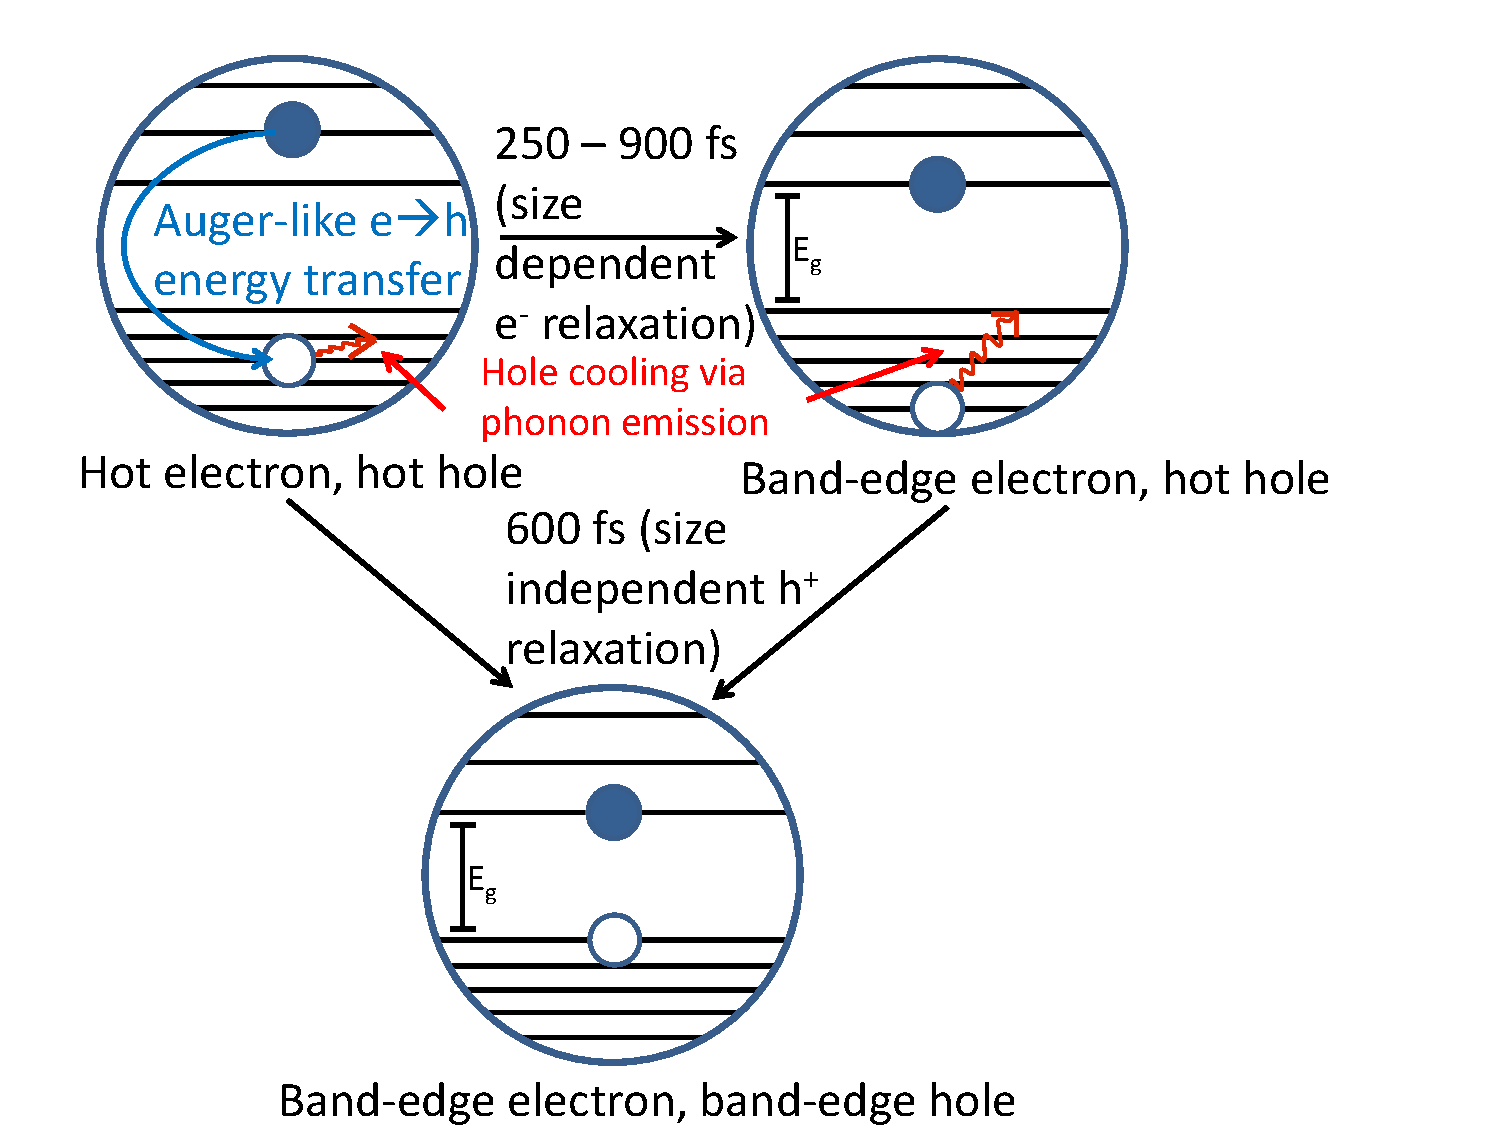
\includegraphics[width=\textwidth]{./Chapter2/fsrs4.pdf}
\caption[Schematic depiction of carrier thermalization in CdSe NCs.]{Following photoexcitation, Auger energy transfer provides the primary relaxation pathway for the electron. Auger energy transfer rates are dependent on NC size. Conversely, hole cooling is primarily facilitated by LO phonon generation, a process with little or no dependence on NC size for CdSe.}
\label{f:fsrs4}
\end{center}
\end{figure}

\section{Electron-Phonon Thermalization in Metallic Nanostructures}
\subsection{Introduction}
While the majority of this thesis is focused on semiconductor systems, we have also explored analogous thermalization processes in small ($\sim$4 nm diameter) gold nanoparticles (Au NPs).  Specifically, we have utilized \emph{ab-initio} atomistic modeling to study the impact of surface chemistry on electron-phonon thermalization in these systems. Overall, we find that electron-phonon thermalization lifetimes (hereafter referred to as $\tau_{ep}$) vary by $\sim$20\% as a function of surface chemistry for otherwise identical systems. Our electronic structure calculations permit us to attribute this variance to an increased electronic heat capacity owing to modification of the DOS near the Fermi level of gold ($E_F$).  

\subsection{Background and Experimental Results}
Numerous existing works suggest a possible impact of chemical passivation on the lifetime of hot electrons in Au NPs \cite{westcott2001adsorbate,hu2002heat,huang2007effect,link2002hot,shin2003comparative}, but the specific mechanism by which the surrounding environment influences the thermalization of hot electrons remains unclear. \par

As a representative example, Figure \ref{f:gold1} shows the transient absorption spectra of 0.7 $\mu$M solutions of aminated and thiolated Au NP samples in toluene at a series of time delays following photoexcitation. These spectra were acquired under pump fluences adjusted to fix the average number of absorbed photons per particle, $\left\langle N\right\rangle$, after accounting for differences in the extinction coefficient between the two samples. Experimental work in this section was carried out by Kenneth Aruda and Christina Sweeney (Department of Chemistry, Northwestern University), and further experimental details may be found in the work by Aruda \emph{et al} \cite{aruda2013identification}. \par

\begin{figure}
\begin{center}
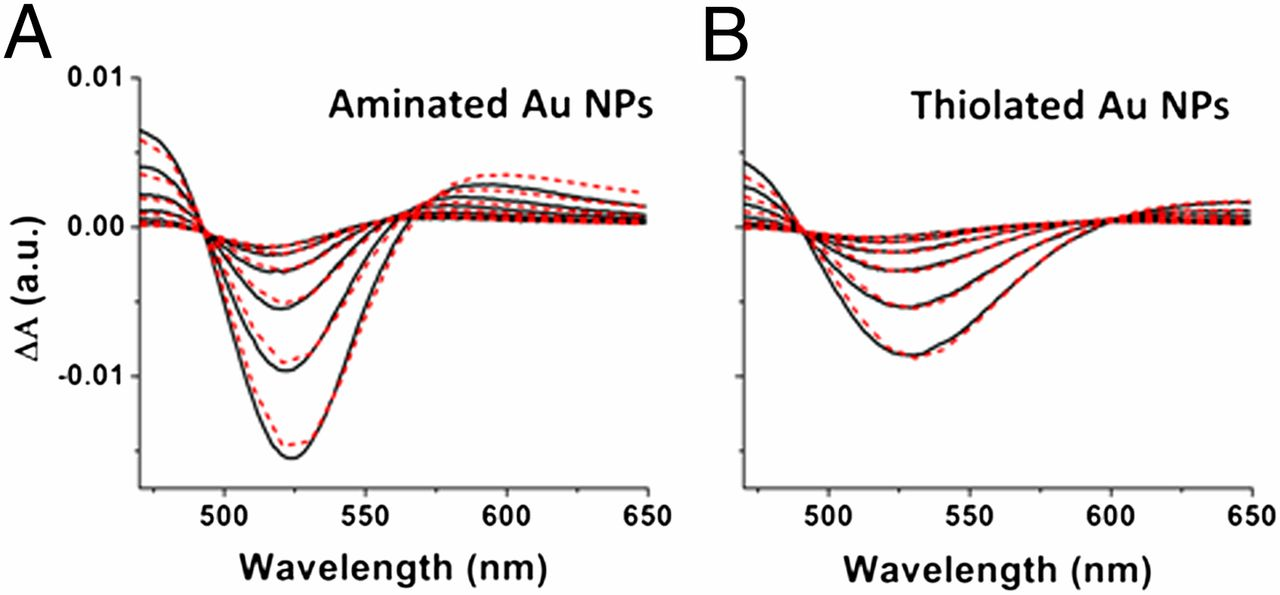
\includegraphics[width=\textwidth]{./Chapter2/gold1.jpg}
\caption[Representative transient absorption spectra of aminated and thiolated Au NP samples.]{Representative transient absorption spectra of aminated (A) and thiolated (B) Au NP samples ($\left\langle N\right\rangle = 2$ photons per particle) at a series of time delays after photoexcitation: 1.5 - 4.5 ps, with 0.6 ps intervals. The dashed red lines are the best fits to each differential spectrum with temperature dependent Mie theory using fixed and floating parameters, as described in the work by Aruda \emph{et al.} \cite{aruda2013identification} From each fit the electronic temeperature of the system may be extracted for the corresponding time delay. Transient absorption data courtesy of Ken Aruda, Weiss lab, Department of Chemistry, Northwestern University.}
\label{f:gold1}
\end{center}
\end{figure}

The time dependence of the TA spectrum can be converted to a time-dependent electronic temperature via fitting of the spectra to temperature-dependent Mie theory \cite{scaffardi2006size,rosei1973d,inouye1998ultrafast}. While the details of the fitting procedure are reported in the literature \cite{aruda2013identification}, the results are summarized in Figure \ref{f:gold2}. Figure \ref{f:gold2} displays the time-dependent electronic temperature following photoexcitation for aminated and thiolated Au NPs. Previous work on electronic cooling in gold has determined that the dynamics on the 300 fs timescale correspond to electron-electron thermalization, while dynamics on the 1-5 ps timescale correspond to thermalization between electronic and vibrational degrees of freedom in the system. Longer decays reflect the dissipation of heat into the solvent bath \cite{link2002hot}. \par

\begin{figure}
\begin{center}
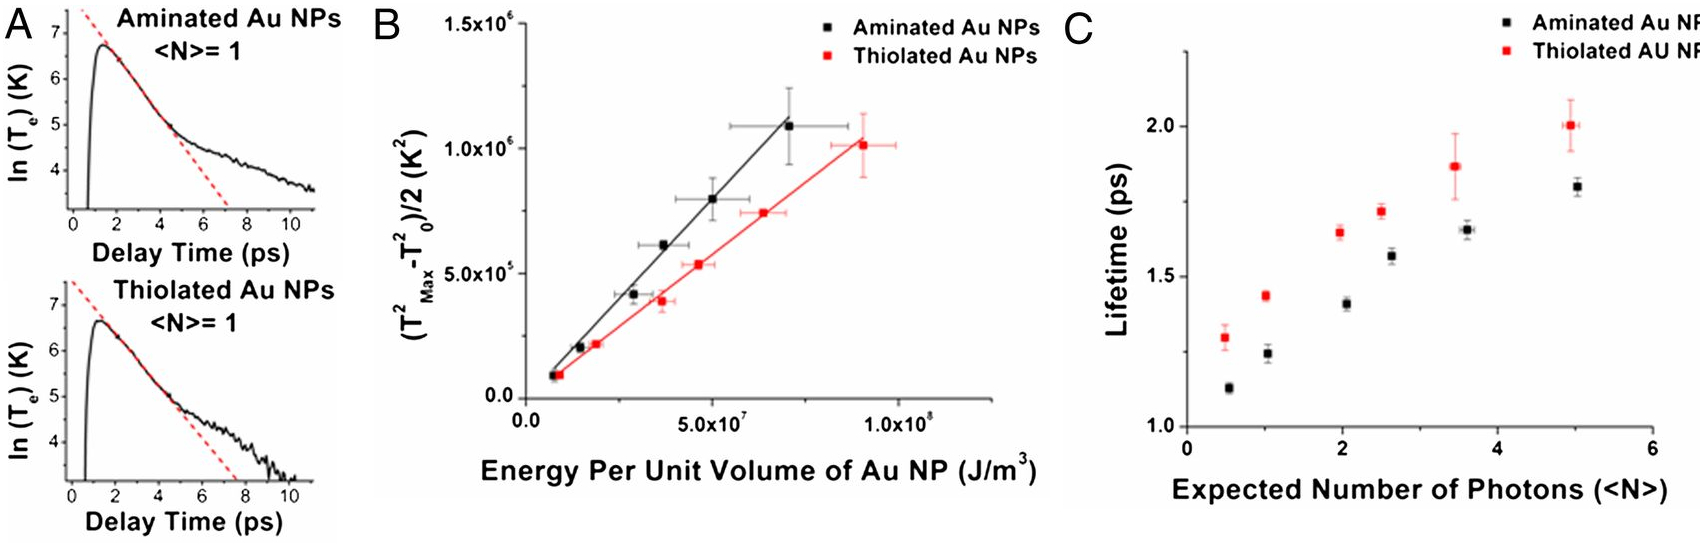
\includegraphics[width=\textwidth]{./Chapter2/gold2.jpg}
\caption[Measurements of hot electron cooling parameters for thiolated and aminated gold nanoparticles.]{(A) The electronic temperature of the thiolated (top) and aminated (bottom) Au NP-ligand systems, determined by fitting the TA spectra as a function of time (\ref{f:gold1}). The kinetic traces show an initial thermalization period caused by electron-electron scattering ($t < 300$ fs) followed by a period in which the hot electron gas equilibrates with vibrational degrees of freedom in the system ($t = 1-5$ ps), and a final period in which the vibrational modes associated with the Au NP dissipate energy into the solvent. The red lines display linear fits to the electron-phonon thermalization regime assuming a first-order decay of the electronic temperature. (B) The square of the initial electronic temperature of the system (following electron-electron scattering) minus the square of the electronic temperature prior to photoexcitation, plotted against the energy of laser normalized by Au NP volume. The slope of this line is inversely proportional to the electronic heat capacity constant for the Au NPs (see Equation \ref{eq:goldeq1}). (C) The observed electron-phonon thermalization lifetime ($\tau_{ep}$) as a function of $\left\langle N\right\rangle$. Expectation values were calculated assuming extinction coefficients of 4.71 $\times$ $10^6$ M$^{-1}$cm$^{-1}$ for the aminated NPs and 3.07 $\times$ $10^6$ M$^{-1}$cm$^{-1}$ for the thiolated NPs at 520 nm. Transient absorption data courtesy of Ken Aruda, Weiss lab, Department of Chemistry, Northwestern University.}
\label{f:gold2}
\end{center}
\end{figure}

The dynamics in Figure \ref{f:gold2}(a) allow us to extract the electronic heat capacity of the system, $\gamma T_e$, where $\gamma$ is the electronic heat capacity coefficient and $T_e$ is the electronic temperature. Experimentally, the electronic heat capacity is related to the energy absorbed by the laser pulse, $U$, \emph{via} $T_e^{max}$, which is the temperature of the electronic system immediately following electron-electron thermalization: \par
\begin{equation}\label{eq:goldeq1}
U = \int_{T_0}^{T_e^{max}}\gamma T_e \mathrm{d}T_e = \frac{1}{2}\gamma(T_e^{max^2} - T_0^2)
\end{equation}
In Eq. \ref{eq:goldeq1}, $T_0$ = 298 K, the initial temperature of the system. Figure \ref{f:gold2}(b) displays the maximum increase in electronic temperature for given values of $U$ for aminated and thiolated Au NPs. These results reveal an elevated $T_e^{max}$ for aminated particles. Given that $T_e^{max}$ is inversely proportional to $\gamma$ (see Eq. \ref{eq:goldeq1}), these results suggest an elevated heat capacity for thiolated particles. \par

Fitting the dynamics in Fig. \ref{f:gold2}(a) to a first-order exponential decay, we may extract the electron-phonon thermalization time constant, $\tau_{ep}$. These extracted lifetimes are displayed as a function of $\left\langle N\right\rangle$ in Fig. \ref{f:gold2}(c). Electron-phonon thermalization times are systematically elevated by $\sim$20\% for thiolated particles relative to aminated particles.

\subsection{Computational Modeling}
In an effort to understand the physical mechanism underlying surface-based modification of the electronic heat capacity, we performed DFT calculations on thiolated and aminated Au slabs.  To prepare initial geometries for DFT calculations, a 5-layer slab of fcc gold having an exposed (111) surface was passivated in four sites on the surface with either methylamine or ethylthiolate. In the methylamine case, the binding geometry found by Trout \emph{et al.} for a gold surface was used as a starting point for the geometry relaxation \cite{pong2005first}. In the case of ethylthiolate, ligands were bound to the (111) surface through a gold ad-atom in a "staple" motif, known to be an extremely stable binding arrangement for both Au (111) surfaces and Au NPs \cite{voznyy2009c,pensa2012chemistry}. Carbon and hydrogen atom positions were initially relaxed using molecular mechanics with the universal force field, as implemented in the Avogadro 1.1.0 software \cite{hanwell2012avogadro}. Following relaxation of the C and H positions, the surfaces of the gold slab with ligands were relaxed within the DFT framework as implemented in the Amsterdam Density Functional (ADF) 2010.01 program. Specifically, atomic positions were relaxed until the force on each atom was less than 0.02 eV/\r{A}, with gold atoms beneath the first two surface layers having fixed positions. All electronic structure calculations utilized the BP86-D GGA exchange correlation functional with a triple-zeta potential basis set having a single polarization function.  To describe core electrons in gold atoms, a 4f frozen core approximation was applied and scalar relativistic effects were incorporated using the zeroth-order regular approximation. In all density of states (DOS) plots, the Fermi level of gold has been set as the zero of energy.  Electronic structure calculations yield a "stick" spectrum of discrete eigenvalues, which are broadened using a Gaussian broadening function with a width of 0.02 eV to yield the DOS spectra reported here. \par

\begin{figure}
\begin{center}
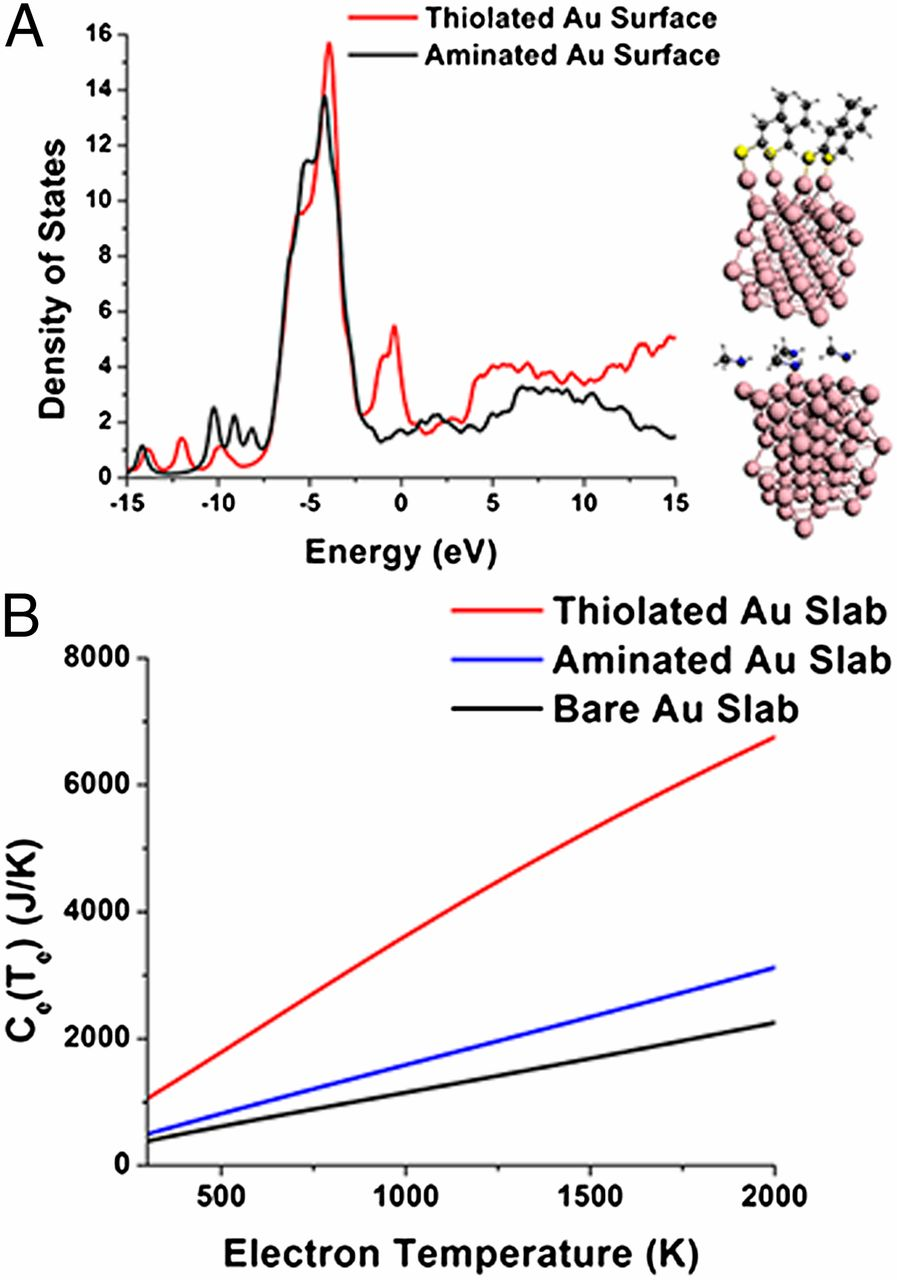
\includegraphics[width=0.5\textwidth]{./Chapter2/gold3.jpg}
\caption[Electronic structure calculations on Au-ligand model systems.]{(A) Density of electronic states as a function of energy for the Au slabs passivated with amines and thiolates (Right). Note that the aminated and thiolated clusters have different state density at the Fermi level (0 eV). Each surface atom on the Au slab is bound to a ligand, such that each cluster in the simulation has the same number of ligands. (B) Calculated electronic heat capacities for the ligated Au slabs in A reproduce the linear dependence of heat capacity on temperature predicted by Eq. \ref{eq:goldeq2}, as well as a dependence of the electronic heat capacity on the electronic DOS at the Fermi level of the Au NP-ligand system.}
\label{f:gold3}
\end{center}
\end{figure}

Figure \ref{f:gold3}(a) shows the electronic DOS of Au slabs functionalized with thiols and amines calculated with DFT. Figure \ref{f:gold3}(b) shows a calculation of the electronic heat capacity, $C_e(T_e)$ for amine- and thiolate-passivated Au slabs using the DFT-derived electronic DOS along with a semiclassical expression for electronic heat capacity as follows \cite{lin2008electron}:
\begin{equation}\label{eq:goldeq2}
C_e(T_e) = \int_{-\infty}^{\infty}\frac{\mathrm{d}f(\varepsilon,\mu,T_e)}{\mathrm{d}T_e}DOS(\varepsilon)\varepsilon\mathrm{d}\varepsilon
\end{equation}
In Eq. \ref{eq:goldeq2}, the function $f(\varepsilon, \mu, T_e)$ is the Fermi-Dirac distribution as a function of energy ($\varepsilon$), chemical potential ($\mu$), and electronic temperature ($T_e$). The results in Fig. \ref{f:gold3}(b) show that the heat capacity for thiolated Au NPs is roughly twice that displayed by the aminated Au NPs, as expected from the increased DOS in the vicinity of the Fermi level (Fig. \ref{f:gold3}(a)) and in general agreement with the results presented in Fig. \ref{f:gold2}. However, quantitative comparisons with experiment are complicated by the elevated ligand-to-gold ratio in the thin slab model used here relative to the Au NPs studied experimentally. The more modest increase in electronic heat capacity observed experimentally may also be understood by considering the effect of electronic structure modifications on electron-phonon coupling. \par

From these electronic structure calculations, we are also able to explore the impact of electronic DOS on the temperature-dependent electron-phonon coupling, $G(T_e)$, as expressed in Equation \ref{eq:goldeq3}:
\begin{equation}\label{eq:goldeq3}
G(T_e) = \frac{\pi\hbar k_B\lambda\left\langle\omega^2\right\rangle}{DOS(E_F)}\int_{-\infty}^{\infty}\frac{\mathrm{d}f(\varepsilon,\mu,T_e)}{\mathrm{d}\varepsilon}DOS^2(\varepsilon)\mathrm{d}\varepsilon
\end{equation}
In Eq. \ref{eq:goldeq3}, $\left\langle\omega^2\right\rangle$ is the second moment of the phonon spectrum and $\lambda$ is the electron-phonon mass enhancement parameter; both parameters are material dependent and assumed here to be bulk Au values. Figure \ref{f:gold4} shows the calculated electron-phonon coupling constants for bare, aminated, and thiolated Au slabs. The thiolated gold slabs, possessing an elevated DOS near $E_F$, exhibit a larger coupling constant than either bare or aminated surfaces. Intuitively, one expects that elevated electron-phonon coupling should facilitate more rapid electron-phonon thermalization, partially offsetting the effects of elevated electronic heat capacity described above.

\begin{figure}
\begin{center}
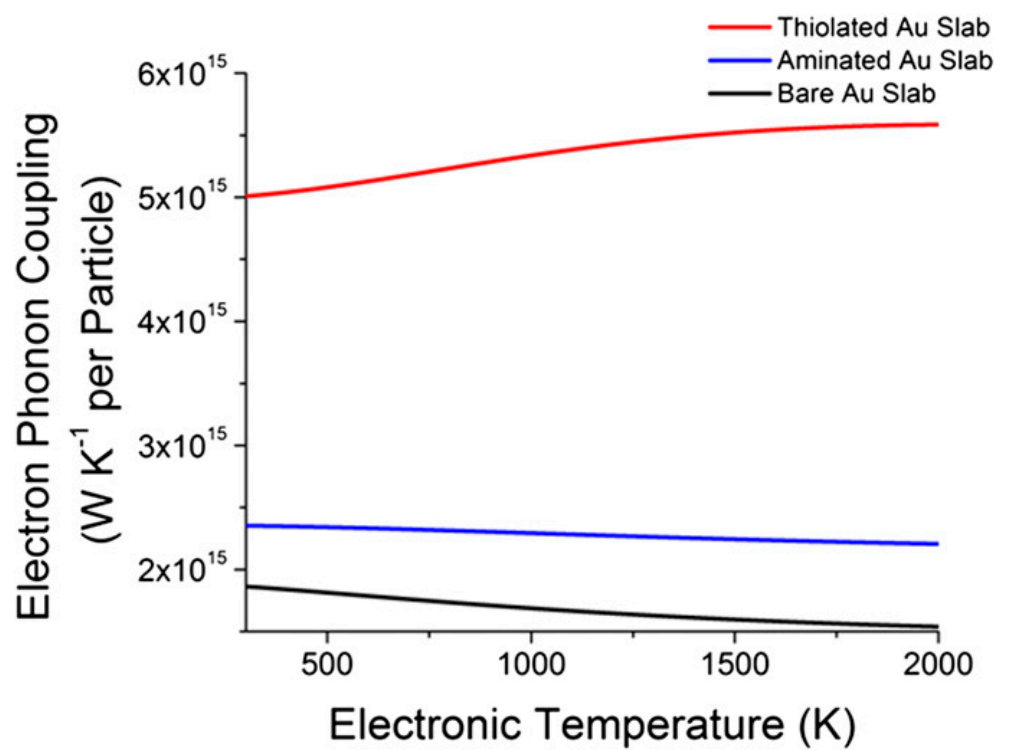
\includegraphics[width=0.75\textwidth]{./Chapter2/gold4.png}
\caption[Simulated electron-phonon coupling constants for thiolated and aminated Au slabs as a function of temperature.]{Simulations of the electron-phonon coupling constant calculated with the electronic density of states determined by DFT of gold slabs. The thiolated
Au slabs with higher DOS at the Fermi level show a larger electron-phonon coupling than both the aminated and bare Au slabs.}
\label{f:gold4}
\end{center}
\end{figure}

\subsection{Conclusions}
Electronic structure calculations were used to explore the impact of surface chemistry on electronic heat capacity and electron-phonon coupling in nanoscale gold structures, which exhibit a dependence (previously) poorly understood dependence on the identity of the passivating chemical species. Motivated by transient absorption measurements demonstrating elevated electron-phonon thermalization times for thiol-passivated Au NPs as compared to aminated Au NPs, we carried out DFT calculations on model Au systems passivated by both types of ligands. These results permit an \emph{ab-initio} calculation of the electronic heat capacity and electron-phonon coupling constant. Thiolated Au slabs were found to exhibit a much larger density of states in the vicinity of the Fermi level, resulting in an elevated electronic heat capacity and electron-phonon coupling constant (see Eqs. \ref{eq:goldeq2} and \ref{eq:goldeq3}).

The larger electronic heat capacity of thiolated Au NPs translates into a smaller driving force for energy exchange between electron and vibrational populations for a given initial electron temperature, and therefore a slower electron cooling process, for thiolated NPs than for aminated NPs. This effect is counteracted by the larger electron-phonon coupling for thiolated NPs than aminated NPs, because electron-phonon coupling increases the rate of energy transfer from electronic states to vibrational states. The increase in both $g$ and $\gamma$ upon exchanging amines for thiolates is not coincidental; both quantities are positively correlated with the electronic DOS near the Fermi level of the NP-ligand system. Overall, our calculations provide microscopic insight into the physical mechansims underlying the observed $\sim$20\% increase in electron-phonon thermalization times in thiol-covered Au NPs.
